%% %%%%%%%%%%%%%%%%%%%%%%%%%%%%%%%%%%%%%%%%%%%%%%%%%%%%%%%%%%%%%%%%%%%%%%%%%%%
%%
%%          $Id: score_sheets.tex 432 2013-05-21 15:33:27Z stueckler $
%%    author(s): RoboCup@Home Technical Committee
%%  description: RoboCup@Home Rulebook: Score Sheets
%%
%% %%%%%%%%%%%%%%%%%%%%%%%%%%%%%%%%%%%%%%%%%%%%%%%%%%%%%%%%%%%%%%%%%%%%%%%%%%%

\documentclass[11pt, a4paper]{book}

\usepackage{soul}

\input{./setup/packages.tex}

\usepackage{fullpage}
\parindent 0cm
\parskip 0.2cm
\topmargin -1cm
\oddsidemargin -1cm
\evensidemargin -1cm
\textwidth 18cm
\textheight 26cm

\input{./setup/active_version.tex}
\graphicspath{{\YEAR/}{./images/}}
\input{./setup/macros.tex}                        % defined in macros.tex
\input{./setup/abbrevix.tex}                      % for list of abbreviations

\hypersetup{
  pdftitle     = {RoboCup@Home Forms \& Score Sheets},
  pdfsubject   = {RoboCup@Home Forms \& Score Sheets},
  pdfauthor    = {RoboCup@Home Technical Committee},
  pdfkeywords  = {RoboCup, @Home, Rules, Competition},
  pdfstartpage = {1},                 % 
  colorlinks   = true,                % Farbige links
  anchorcolor  = black,               % anchor-text (header)
  linkcolor    = black,               % content,index,ref/pageref-label
  urlcolor     = blue,                % URLs - http-Adressedate (auch TeX)
  pdfcreator   = {pdflatex},
  pdfproducer  = {latex-pdftex}
}

%% %%%%%%%%%%%%%%%%%%%%%%%%%%%%%%%%%%%% %%
%%  H E A D I N G S                     %%
%% %%%%%%%%%%%%%%%%%%%%%%%%%%%%%%%%%%%% %%

%% * Pagestyle
\fancypagestyle{plain}{
        \fancyhf{}
        \fancyhead{}
        \fancyfoot[C]{\scriptsize \sffamily \footline{}}
		\renewcommand{\headrulewidth}{0 pt}
}

\newcommand{\footline}{RoboCup@Home Forms \& Score Sheets / \rulebookVersion}



\begin{document}

\input{teams.tex}

\begin{titlepage}
  \begin{center}
    {
      \includegraphics[width=.25\textwidth]{images/logo_RoboCupFed.jpg}
      \hfill
      \includegraphics[width=.25\textwidth]{images/logo_RoboCupAtHome.jpg}\\[1.23ex]
    }
    \vspace{2.7 cm}
    \hrulefill\par
    {%
      \vspace*{.27cm}
      \Huge{RoboCup@Home}\\[1.23ex]
      \Large Forms \& Score Sheets\\[2ex]
    }
    \hrulefill\par
    \vfill
    ~~ Version: \YEAR \quad \svnRevision ~~ \\
    ~~ Last Build Date: \today \quad Time: \the\time ~~ \\
    ~~ \svnChangeData ~~ %\\
    %\vfill
  \end{center}
\end{titlepage}

\pagestyle{plain}

\input{registration_form.tex}

\renewcommand{\shortScoresheet}{false}

% \TODO{Write new score sheets}

\renewcommand{\currentTest}{Poster Session}
\renewcommand{\retryAvailable}{false}
\renewcommand{\continueAvailable}{false}
\begin{scoresheet}
\input{scoresheets/PosterSession}
\end{scoresheet}

%% %%%%%%%%%%%%%%%%%%%%%%%%%%%%%%%%%%%%%%%%%%%%%%%%%%%%%%%%%%%%%%%%%%%%%%% %%
%%                                                                         %%
%% STAGE I                                                                 %%
%%                                                                         %%
%% %%%%%%%%%%%%%%%%%%%%%%%%%%%%%%%%%%%%%%%%%%%%%%%%%%%%%%%%%%%%%%%%%%%%%%% %%

\renewcommand{\retryAvailable}{false}
\renewcommand{\continueAvailable}{true}
\renewcommand{\threeAttempts}{true}
%%% STAGE 1 TESTS GO HERE %%%

% Cocktail Party
% \renewcommand{\currentTest}{Cocktail Party}
% \begin{scoresheet}
% \input{scoresheets/CocktailParty.tex}
% \end{scoresheet}

% GPSR
\renewcommand{\currentTest}{General Purpose Robot}
\begin{scoresheet}
\input{scoresheets/GPSR.tex}
\end{scoresheet}

% Help-me-carry
\renewcommand{\currentTest}{Help-me-carry}
\begin{scoresheet}

The maximum time for this test is 6 minutes.

\begin{scorelist}
	\scoreheading{Single iteration}
	\scoreitem{10}{Reach the car}
	\scoreitem{20}{Natural handover to accept the item from the owner}
	\scoreitem{5}{Understand the commanded destination}
	\scoreitem{10}{Reach inside the arena again}
	\scoreitem{10}{Reach the destination}
	\scoreitem{5}{Put the item at the floor or a nearby table}
	% 3x 60 points = 180 only
	
	% Up to 60 points
	\scoreheading{Dealing with obstacles}
	\scoreitem{5}{Avoiding small object}
	\scoreitem{10}{Avoiding 3D object (Difficult-to-see object)}
	\scoreitem{5}{Asking a person to step aside}
	\scoreitem{30}{Moving away movable object}
	\scoreitem{10}{Move aside for person}
	\scoreitem{50}{Open closed door}
	
	\setTotalScore{290}
\end{scorelist}


% Local Variables:
% TeX-master: "Rulebook"
% End:

\end{scoresheet}

% Speech and Person Recognition
\renewcommand{\continueAvailable}{false}
\renewcommand{\currentTest}{Speech and Person Recognition}
\begin{scoresheet}
\input{scoresheets/SPR.tex}
\end{scoresheet}
\renewcommand{\continueAvailable}{true}

% Storing Groceries
\renewcommand{\currentTest}{Storing Groceries}
\begin{scoresheet}
\section{Storing Groceries}

The robot must store the groceries on their right place, which is where other objects of the same category are.

\subsection{Goal}
The robot has to correctly identify and manipulate objects at different heights, grouping them by category and likelihood.

\subsection{Focus}
This test focuses on the detection and recognition of objects and their features, as well as object manipulation.

\subsection{Setup}
\begin{enumerate}
\item \textbf{Location:} This test is run in one room of the arena, modified to have a table or trolley (at grasp distance) close to a shelf. The robot will start at a random distance between 1.0m and 1.5m from the bookcase.
\item \textbf{Cupboard:} Any shelf from the arena allocating 10 objects (3 known, 3 alike, 3 unknown, 1 container; see \ref{rule:scenario_objects}) grouped by category and likeliness. 
\item \textbf{Door:} The cupboard has a single door, which is initially closed. At least one object group is accessed through the door.
\item \textbf{Table:} Any table from the arena, having on top 10 shuffled objects (probably stacked, 3 known, 3 alike, 3 unknown, 1 container; see \ref{rule:scenario_objects})
\end{enumerate}

Please note that there may be more than one object in each shelf to fit all objects in, especially after the robot fills the shelves. 

\subsection{Task}
\begin{enumerate}
\item \textbf{Reach the cupboard:} The robot approached to the cupboard (and the table) at grasp distance.
\item \textbf{Inspection:} The robot inspects both, the cupboard and the table.
\item \textbf{Opening door:} The robot opens the cupboard's door and announces which type of objects are stored inside.
\item \textbf{Moving objects:} The robot takes an object from the table and safely places it into the shelf (see Section \refsec{rule:scenario_objects}), close to the other objects in the shelf that belong to the same category. The robot must clearly announce the name and category of the object being moved.
\end{enumerate}

\subsection{Additional rules and remarks}
\begin{enumerate}
  \item \textbf{Startup:} The robot starts with a Start Button (see Section \refsec{rule:start_signal})
  \item \textbf{Collisions:} Slightly touching the the cupboard is tolerated. However, the robot will be stopped immediately if it drives over or smashes the objects/shelf (see section \refsec{rule:safetyfirst}).
  \item \textbf{Cupboard specifications:} The cupboard is any shelf from the arena and has
  \begin{itemize}
    \item[\textbf{DSPL}] At least 3 shelves between 0.90m and 1.50m from the ground.
    \item[\textbf{SSPL}] At least 3 shelves between 0.90m and 1.50m from the ground.
    \item[\textbf{OPL}] At least 5 shelves between 0.30m and 1.80m from the ground.
  \end{itemize}
  \item \textbf{Cupboard's door specifications:} The cupboard has a door that opens outside (i.e., not sliding). The door has a handle or knob is coloured to contrast with the shelve.
  \item \textbf{Recognition report:} Robots must create a report file in PDF format summarizing the the list of recognized objects, and containing the following information:
  \begin{itemize}
    \item A picture of the scene where all recognized objects are labeled and enclosed in a bounding box.
    \item A picture showing each object, it's name/label, and category.
  \end{itemize}

  The report file must be delivered to the TC in a USB-stick after the test. The PDF file name should include the team name and a timestamp.  Objects in the report must be recognizable by a human (TC) so that it can be scored. In case of doubt, no points will be scored.
  \item \textbf{Clear area: } The robot may assume that the direct vicinity of the cupboard and table are clear and that the robot can move slightly backwards for its task. 
\end{enumerate}

\subsection{Data recording}
  Please record the following data (See \refsec{rule:datarecording}):
  \begin{itemize}
   \item Images
   \item Plans
  \end{itemize}

\subsection{OC instructions}

\textbf{2 hours before the test}
\begin{itemize}
    \item Anounce the startup location for robots.
\end{itemize}

\subsection{Referee instructions}
The referee needs to
\begin{itemize}
\item Place the objects in the cupboard and on the table.
\item Shut the cupboard's door.
\end{itemize}

\begin{figure}
  \centering
  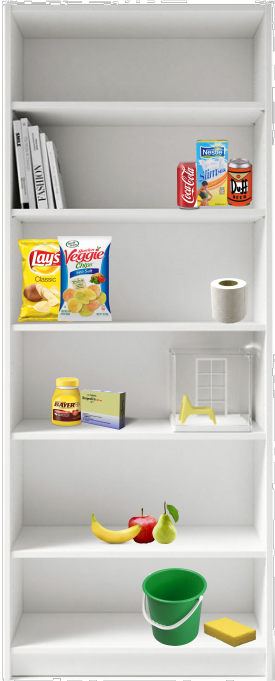
\includegraphics[width=0.25\textwidth]{images/storing_groceries.png}
  \vspace{-10pt}
  \label{fig:storing_groceries}
  \caption{Example shelf where objects will be placed.}
\end{figure}

\subsection{Score sheet}
\section{Storing Groceries}

The robot must store the groceries on their right place, which is where other objects of the same category are.

\subsection{Goal}
The robot has to correctly identify and manipulate objects at different heights, grouping them by category and likelihood.

\subsection{Focus}
This test focuses on the detection and recognition of objects and their features, as well as object manipulation.

\subsection{Setup}
\begin{enumerate}
\item \textbf{Location:} This test is run in one room of the arena, modified to have a table or trolley (at grasp distance) close to a shelf. The robot will start at a random distance between 1.0m and 1.5m from the bookcase.
\item \textbf{Cupboard:} Any shelf from the arena allocating 10 objects (3 known, 3 alike, 3 unknown, 1 container; see \ref{rule:scenario_objects}) grouped by category and likeliness. 
\item \textbf{Door:} The cupboard has a single door, which is initially closed. At least one object group is accessed through the door.
\item \textbf{Table:} Any table from the arena, having on top 10 shuffled objects (probably stacked, 3 known, 3 alike, 3 unknown, 1 container; see \ref{rule:scenario_objects})
\end{enumerate}

Please note that there may be more than one object in each shelf to fit all objects in, especially after the robot fills the shelves. 

\subsection{Task}
\begin{enumerate}
\item \textbf{Reach the cupboard:} The robot approached to the cupboard (and the table) at grasp distance.
\item \textbf{Inspection:} The robot inspects both, the cupboard and the table.
\item \textbf{Opening door:} The robot opens the cupboard's door and announces which type of objects are stored inside.
\item \textbf{Moving objects:} The robot takes an object from the table and safely places it into the shelf (see Section \refsec{rule:scenario_objects}), close to the other objects in the shelf that belong to the same category. The robot must clearly announce the name and category of the object being moved.
\end{enumerate}

\subsection{Additional rules and remarks}
\begin{enumerate}
  \item \textbf{Startup:} The robot starts with a Start Button (see Section \refsec{rule:start_signal})
  \item \textbf{Collisions:} Slightly touching the the cupboard is tolerated. However, the robot will be stopped immediately if it drives over or smashes the objects/shelf (see section \refsec{rule:safetyfirst}).
  \item \textbf{Cupboard specifications:} The cupboard is any shelf from the arena and has
  \begin{itemize}
    \item[\textbf{DSPL}] At least 3 shelves between 0.90m and 1.50m from the ground.
    \item[\textbf{SSPL}] At least 3 shelves between 0.90m and 1.50m from the ground.
    \item[\textbf{OPL}] At least 5 shelves between 0.30m and 1.80m from the ground.
  \end{itemize}
  \item \textbf{Cupboard's door specifications:} The cupboard has a door that opens outside (i.e., not sliding). The door has a handle or knob is coloured to contrast with the shelve.
  \item \textbf{Recognition report:} Robots must create a report file in PDF format summarizing the the list of recognized objects, and containing the following information:
  \begin{itemize}
    \item A picture of the scene where all recognized objects are labeled and enclosed in a bounding box.
    \item A picture showing each object, it's name/label, and category.
  \end{itemize}

  The report file must be delivered to the TC in a USB-stick after the test. The PDF file name should include the team name and a timestamp.  Objects in the report must be recognizable by a human (TC) so that it can be scored. In case of doubt, no points will be scored.
  \item \textbf{Clear area: } The robot may assume that the direct vicinity of the cupboard and table are clear and that the robot can move slightly backwards for its task. 
\end{enumerate}

\subsection{Data recording}
  Please record the following data (See \refsec{rule:datarecording}):
  \begin{itemize}
   \item Images
   \item Plans
  \end{itemize}

\subsection{OC instructions}

\textbf{2 hours before the test}
\begin{itemize}
    \item Anounce the startup location for robots.
\end{itemize}

\subsection{Referee instructions}
The referee needs to
\begin{itemize}
\item Place the objects in the cupboard and on the table.
\item Shut the cupboard's door.
\end{itemize}

\begin{figure}
  \centering
  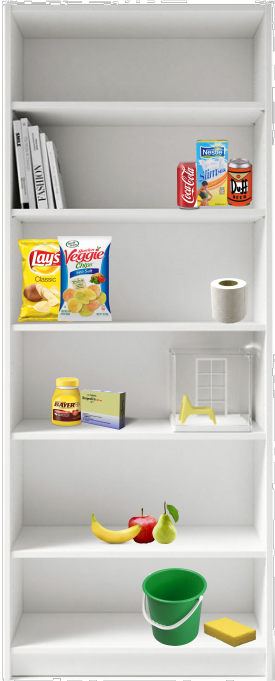
\includegraphics[width=0.25\textwidth]{images/storing_groceries.png}
  \vspace{-10pt}
  \label{fig:storing_groceries}
  \caption{Example shelf where objects will be placed.}
\end{figure}

\subsection{Score sheet}
\section{Storing Groceries}

The robot must store the groceries on their right place, which is where other objects of the same category are.

\subsection{Goal}
The robot has to correctly identify and manipulate objects at different heights, grouping them by category and likelihood.

\subsection{Focus}
This test focuses on the detection and recognition of objects and their features, as well as object manipulation.

\subsection{Setup}
\begin{enumerate}
\item \textbf{Location:} This test is run in one room of the arena, modified to have a table or trolley (at grasp distance) close to a shelf. The robot will start at a random distance between 1.0m and 1.5m from the bookcase.
\item \textbf{Cupboard:} Any shelf from the arena allocating 10 objects (3 known, 3 alike, 3 unknown, 1 container; see \ref{rule:scenario_objects}) grouped by category and likeliness. 
\item \textbf{Door:} The cupboard has a single door, which is initially closed. At least one object group is accessed through the door.
\item \textbf{Table:} Any table from the arena, having on top 10 shuffled objects (probably stacked, 3 known, 3 alike, 3 unknown, 1 container; see \ref{rule:scenario_objects})
\end{enumerate}

Please note that there may be more than one object in each shelf to fit all objects in, especially after the robot fills the shelves. 

\subsection{Task}
\begin{enumerate}
\item \textbf{Reach the cupboard:} The robot approached to the cupboard (and the table) at grasp distance.
\item \textbf{Inspection:} The robot inspects both, the cupboard and the table.
\item \textbf{Opening door:} The robot opens the cupboard's door and announces which type of objects are stored inside.
\item \textbf{Moving objects:} The robot takes an object from the table and safely places it into the shelf (see Section \refsec{rule:scenario_objects}), close to the other objects in the shelf that belong to the same category. The robot must clearly announce the name and category of the object being moved.
\end{enumerate}

\subsection{Additional rules and remarks}
\begin{enumerate}
  \item \textbf{Startup:} The robot starts with a Start Button (see Section \refsec{rule:start_signal})
  \item \textbf{Collisions:} Slightly touching the the cupboard is tolerated. However, the robot will be stopped immediately if it drives over or smashes the objects/shelf (see section \refsec{rule:safetyfirst}).
  \item \textbf{Cupboard specifications:} The cupboard is any shelf from the arena and has
  \begin{itemize}
    \item[\textbf{DSPL}] At least 3 shelves between 0.90m and 1.50m from the ground.
    \item[\textbf{SSPL}] At least 3 shelves between 0.90m and 1.50m from the ground.
    \item[\textbf{OPL}] At least 5 shelves between 0.30m and 1.80m from the ground.
  \end{itemize}
  \item \textbf{Cupboard's door specifications:} The cupboard has a door that opens outside (i.e., not sliding). The door has a handle or knob is coloured to contrast with the shelve.
  \item \textbf{Recognition report:} Robots must create a report file in PDF format summarizing the the list of recognized objects, and containing the following information:
  \begin{itemize}
    \item A picture of the scene where all recognized objects are labeled and enclosed in a bounding box.
    \item A picture showing each object, it's name/label, and category.
  \end{itemize}

  The report file must be delivered to the TC in a USB-stick after the test. The PDF file name should include the team name and a timestamp.  Objects in the report must be recognizable by a human (TC) so that it can be scored. In case of doubt, no points will be scored.
  \item \textbf{Clear area: } The robot may assume that the direct vicinity of the cupboard and table are clear and that the robot can move slightly backwards for its task. 
\end{enumerate}

\subsection{Data recording}
  Please record the following data (See \refsec{rule:datarecording}):
  \begin{itemize}
   \item Images
   \item Plans
  \end{itemize}

\subsection{OC instructions}

\textbf{2 hours before the test}
\begin{itemize}
    \item Anounce the startup location for robots.
\end{itemize}

\subsection{Referee instructions}
The referee needs to
\begin{itemize}
\item Place the objects in the cupboard and on the table.
\item Shut the cupboard's door.
\end{itemize}

\begin{figure}
  \centering
  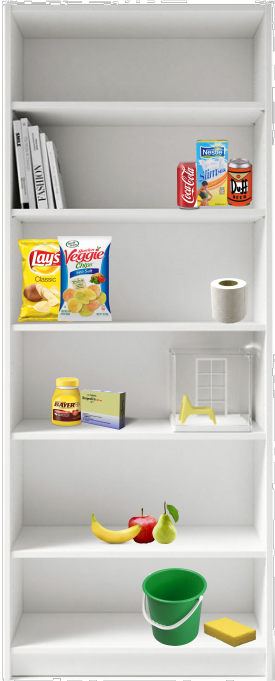
\includegraphics[width=0.25\textwidth]{images/storing_groceries.png}
  \vspace{-10pt}
  \label{fig:storing_groceries}
  \caption{Example shelf where objects will be placed.}
\end{figure}

\subsection{Score sheet}
\input{scoresheets/StoringGroceries.tex}

% Local Variables:
% TeX-master: "Rulebook"
% End:


% Local Variables:
% TeX-master: "Rulebook"
% End:


% Local Variables:
% TeX-master: "Rulebook"
% End:

\end{scoresheet}

%% %%%%%%%%%%%%%%%%%%%%%%%%%%%%%%%%%%%%%%%%%%%%%%%%%%%%%%%%%%%%%%%%%%%%%%% %%
%%                                                                         %%
%% STAGE II                                                                %%
%%                                                                         %%
%% %%%%%%%%%%%%%%%%%%%%%%%%%%%%%%%%%%%%%%%%%%%%%%%%%%%%%%%%%%%%%%%%%%%%%%% %%

\renewcommand{\retryAvailable}{true}
\renewcommand{\continueAvailable}{true}
\renewcommand{\threeAttempts}{false}
%%% STAGE 2 TESTS GO HERE %%%

% EEGPSR
\renewcommand{\currentTest}{EEGPSR}
\begin{scoresheet}
\input{scoresheets/EEGPSR.tex}
\end{scoresheet}

% Open Challenge
\renewcommand{\retryAvailable}{false}
\renewcommand{\continueAvailable}{false}
\renewcommand{\currentTest}{Open challenge}
\begin{scoresheet}
\input{scoresheets/OpenChallenge.tex}
\end{scoresheet}
\renewcommand{\continueAvailable}{true}
\renewcommand{\retryAvailable}{true}

% Restaurant
\renewcommand{\currentTest}{Restaurant}
\begin{scoresheet}
\input{scoresheets/Restaurant.tex}
\end{scoresheet}

%TidyUp
\renewcommand{\currentTest}{TidyUp}
\begin{scoresheet}
\input{scoresheets/TidyUp.tex}
\end{scoresheet}




%% %%%%%%%%%%%%%%%%%%%%%%%%%%%%%%%%%%%%%%%%%%%%%%%%%%%%%%%%%%%%%%%%%%%%%%% %%
%%                                                                         %%
%% FINALS                                                                  %%
%%                                                                         %%
%% %%%%%%%%%%%%%%%%%%%%%%%%%%%%%%%%%%%%%%%%%%%%%%%%%%%%%%%%%%%%%%%%%%%%%%% %%

\renewcommand{\retryAvailable}{false}
\renewcommand{\continueAvailable}{false}
\renewcommand{\threeAttempts}{false}
%%% SCORESHEETS FOR FINALS GO HERE %%%

\renewcommand{\currentTest}{Final Demonstration -- Jury Evaluation}
\begin{scoresheet}
\input{scoresheets/FinalsJury.tex}
\end{scoresheet}

\renewcommand{\currentTest}{Final Demonstration -- Executive Committee}
\begin{scoresheet}
\input{scoresheets/FinalsExec.tex}
\end{scoresheet}

\end{document}

